\documentclass[11pt]{article}
\usepackage[margin=1in]{geometry}
\usepackage{amsmath,amssymb,graphicx}
\usepackage[colorlinks=true,allcolors=blue]{hyperref}
\graphicspath{{../figures/}}
\newcommand{\PP}{\mathbb P}
\newcommand{\SSemi}{\mathcal S_2}
\newcommand{\ones}{\mathbf 1}
\newcommand{\OmegaF}{\Omega}
\newcommand{\sing}{\mathfrak S}
\newcommand{\Var}{\operatorname{Var}}
\title{Supplement: cross-disciplinary reframings of the\\ Goldbach--Chen frontier}
\author{Mathias Rodr\'iguez Castro}
\date{June 2026}
\begin{document}
\maketitle
\noindent This supplement develops the seven cross-disciplinary reframings summarized in
Appendix~C of the main paper, \emph{The Goldbach--Chen Frontier: A Singular-Series
Cancellation Identity and a Bounded Almost-All Reduction}. As explained there, each recasts
the same singular-series governance in a different external language; we keep them, with
their figures and the honest negatives, for the individual vocabularies, not as independent
results. ``The main text'' refers to that paper.
\medskip

\section{Goldbach as arithmetic ground-state energy}
\label{sec:energy-emp}

A single reformulation subsumes the counts $R_1,R_2$, the layers $\OmegaF(q)=k$, and
the partition-function viewpoint. Assign to each decomposition $a+b=N$ ($a,b\ge2$) the
\emph{arithmetic energy} $H(a,b)=\OmegaF(a)+\OmegaF(b)$, and define the ground-state
energy and level spectrum
\[
  E(N)=\min_{a+b=N}H(a,b),\qquad
  n_E(N)=\#\{a+b=N:\ \OmegaF(a)+\OmegaF(b)=E\}.
\]
Then $E(N)=2$ \emph{iff} Goldbach holds for $N$; the ground-state degeneracy is
$n_2(N)=R_1(N)$, and the first excited level is $n_3(N)=2R_2(N)$ (prime$+$semiprime,
Chen). The spectrum (Fig.~\ref{fig:energy}, left) is a hump peaked at the typical energy
$\langle H\rangle\sim2\log\log N$, with the Goldbach ground state sitting in its
low-energy tail; the gap $\langle H\rangle-E(N)\sim2\log\log N-2$ diverges.

The thermodynamics is computable for all $N$ at once, since the partition function is a
self-convolution,
\[
  Z_N(\beta)=\sum_{a+b=N}e^{-\beta H(a,b)}=(f_\beta*f_\beta)(N),\qquad f_\beta(n)=e^{-\beta\OmegaF(n)},
\]
so one FFT per $\beta$ yields $Z_N$, the mean energy $U_N(\beta)=-\partial_\beta\log Z_N$,
and the specific heat $C_N(\beta)=\beta^2\Var_\beta(H)$. As $\beta$ increases past a
``melting'' point $\beta^\star(N)$, the system localises onto the Goldbach ground state:
$U_N$ drops from $\sim2\log\log N$ to $2$ and $C_N(\beta)$ peaks at $\beta^\star$
(Fig.~\ref{fig:energy}, centre; mean $\beta^\star\approx2.1$). Strikingly, this melting
temperature is almost a deterministic function of the singular series:
$\operatorname{corr}(\beta^\star,\log\sing)=-0.92$ (Fig.~\ref{fig:energy}, right). Where
$\sing(N)$ is large the ground state is highly degenerate ($R_1\propto\sing$) and
entropically favoured, so Goldbach order melts at a \emph{lower} $\beta$. Thus the same
singular series that governs $R_1$, $\beta_2$ and the balance exponent also governs the
thermodynamic stability of the Goldbach ground state---a unified statistical-mechanical
picture in which Goldbach is the statement ``every even $N$ has ground-state energy $2$''.

\begin{figure}[h]
\centering
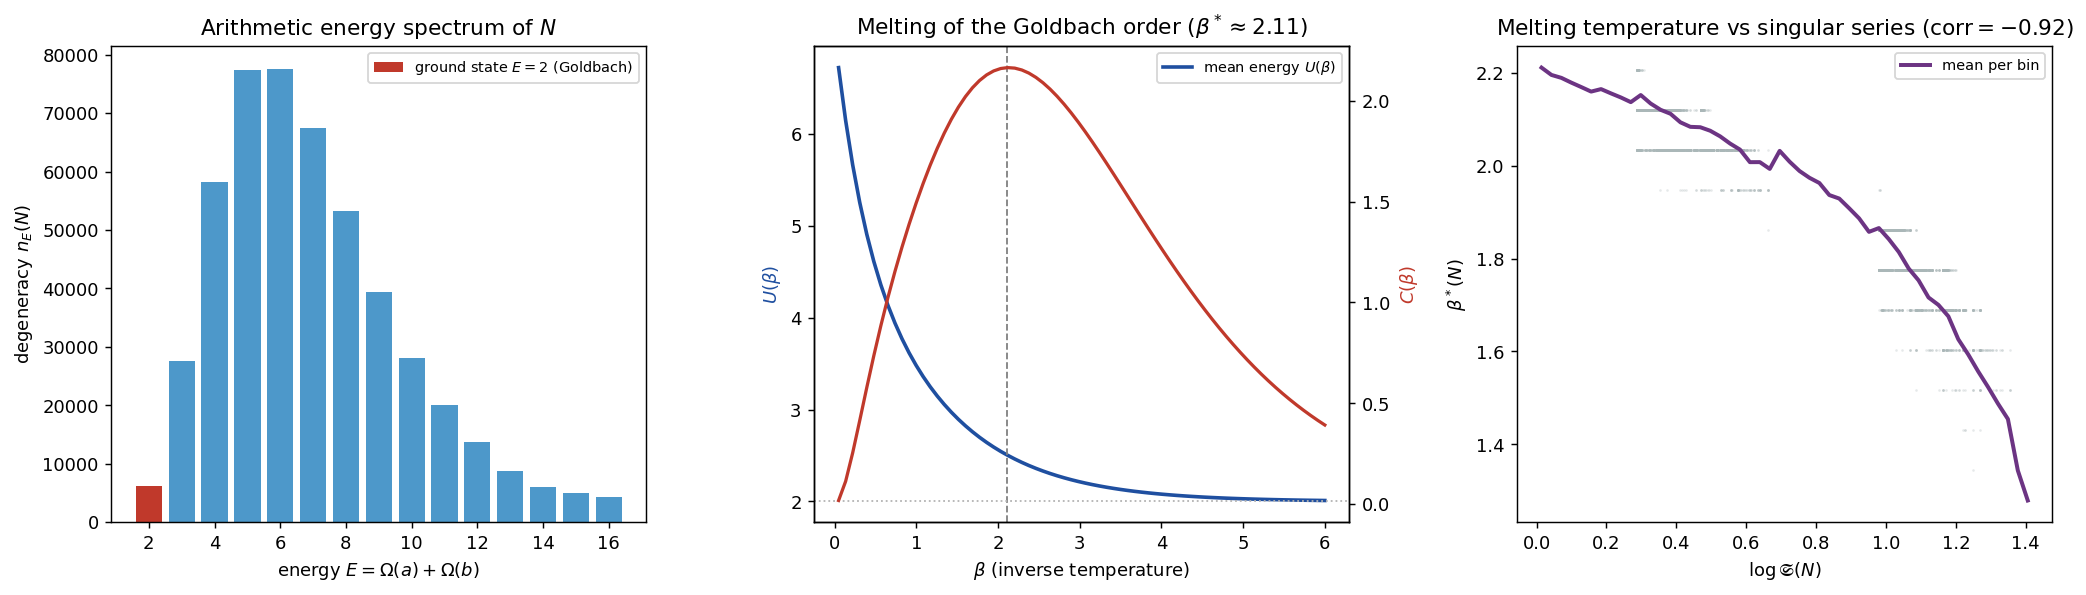
\includegraphics[width=\linewidth]{17_energia.png}
\caption{Arithmetic ground-state energy. Left: the energy spectrum $n_E(N)$, a hump at
$\sim2\log\log N$ with the Goldbach ground state $E=2$ (red) in its tail. Centre: mean
energy $U(\beta)\to2$ and specific heat $C(\beta)$, whose peak $\beta^\star\approx2.1$ is
the melting temperature of Goldbach order. Right: $\beta^\star$ versus $\log\sing(N)$
(correlation $-0.92$).}
\label{fig:energy}
\end{figure}

\section{Adversarial robustness of the Goldbach graph}
\label{sec:robust-emp}

View the representations as a bipartite graph: even integers $N$ on one side, primes
$p$ on the other, with an edge $N\!\sim\!p$ when $N-p$ is prime; the degree of $N$ is
$R_1(N)/2$. How robust is Goldbach to deletion of primes? On a window of $1.5\cdot10^{4}$
even integers near $10^{6}$ we compare three adversaries (Fig.~\ref{fig:robust}).

\emph{Random deletion} is almost powerless: deleting each prime independently with
probability $\phi$ leaves $N$ representable unless all its $\sim R_1(N)/2$ disjoint pairs
are hit, an event of probability $(1-(1-\phi)^2)^{R_1(N)/2}$. Goldbach survives in the
\emph{whole} window until $\phi\approx0.97$; one may delete $95\%$ of all primes at random
and still represent every $N$.

\emph{Targeted deletion} is efficient but local: since the pairs $\{p,N-p\}$ of a fixed
$N$ are disjoint, breaking $N$ is a vertex cover of a matching, costing exactly
$R_1(N)/2$ primes; the cheapest target is the lowest-degree $N$, giving
$\kappa=\min_N R_1(N)/2$. In the window this is $4.6\%$ of the primes---an order of
magnitude less than the random threshold, but aimed at a single $N$.

\emph{Modular deletion} is the striking case. Delete the primes in one reduced class
$a\bmod m$. The survivors lie in $(\mathbb Z/m)^\times\setminus\{a\}$, and an $N$ is
destroyed when its class is missing from the survivors' sumset. For $m=3$, deleting the
class $1$ (i.e.\ \emph{half} of all primes) leaves only the class $2$, whose sumset is
$\{2+2\}=\{1\}$: every $N\equiv0,2\pmod3$ loses all its representations, destroying $59\%$
of the window (Fig.~\ref{fig:robust}, right). The same $50\%$ of primes removed at random
destroys nothing. Thus the adversary manufactures a \emph{local obstruction}---the exact
mechanism the singular series rules out for the primes themselves. The effect is confined
to the smallest moduli: $m=4$ deleting class $1$ kills $N\equiv0\bmod4$ ($50\%$), while for
$m\ge5$ the surviving classes already sum onto everything and no $N$ is fully obstructed.

In short, the Goldbach graph is \emph{random-robust but structure-fragile}: invulnerable to
losing almost all primes by chance, yet shattered by removing one arithmetic progression.
This is a network-science counterpart of the local--global theme: Goldbach's redundancy is
enormous, but it is arithmetic, not statistical, redundancy.

\begin{figure}[h]
\centering
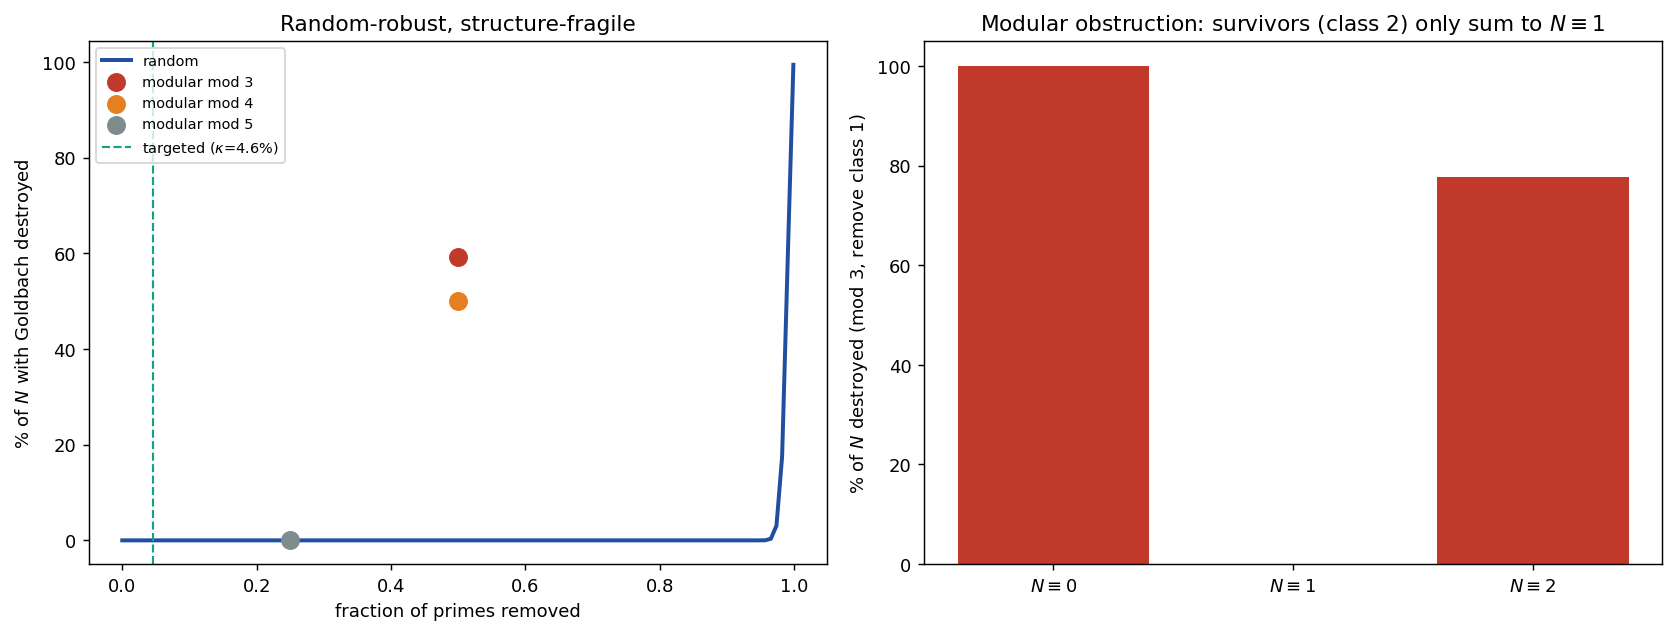
\includegraphics[width=\linewidth]{18_robustez.png}
\caption{Robustness of the Goldbach graph. Left: fraction of window $N$ destroyed versus
fraction of primes deleted---random deletion (curve) only bites near $\phi=1$, whereas the
modular attacks at $\phi=0.5$ (mod $3,4$) destroy $50$--$60\%$, and the targeted cut needs
only $\kappa=4.6\%$. Right: under the mod-$3$ attack, $N\equiv0$ and $N\equiv2$ are
obstructed while $N\equiv1$ is untouched.}
\label{fig:robust}
\end{figure}

\section{Goldbach as a market: liquidity and the fair-weather substitute}
\label{sec:market-emp}

Read each even $N$ as a market that must clear by hiring two prime inputs $p+q=N$; the
liquidity is the number of matches, $L_G(N)=R_1(N)$. Chen lets one input be a
\emph{minimally composite substitute} (a semiprime), giving $L_C(N)=R_1(N)+R_2(N)$ and a
substitute spread $S_C(N)=R_2/R_1\approx2.3$: in normal times the Chen market is three
times more liquid. We ask whether the substitute also provides \emph{resilience} under a
supply shock that removes each prime with probability $\phi$. A Goldbach match survives
with probability $(1-\phi)^2$ (two primes), but a Chen match only with $(1-\phi)^3$,
because the semiprime $q=rs$ needs its two factors $r,s$ to survive as well. Hence the
expected surviving liquidities are $L_G(\phi)=R_1(1-\phi)^2$ and
$L_C(\phi)=L_G(\phi)+R_2(1-\phi)^3$, and the substitute spread \emph{decays linearly},
\[
  S_C(\phi)=\frac{L_C(\phi)-L_G(\phi)}{L_G(\phi)}=S_C(0)\,(1-\phi)\ \longrightarrow\ 0 .
\]
Solving $L(\phi)=1$ for the illiquidity threshold, both markets collapse at essentially the
same point, $\phi_G\approx\phi_C\approx0.989$, and the resilience premium
$\phi_C-\phi_G\approx2\cdot10^{-4}$ is negligible (Fig.~\ref{fig:market}). The economic
reading is clean and a little counter-intuitive: the Chen channel is \emph{fair-weather
liquidity}---abundant when primes are plentiful, but worth ever less precisely as they
become scarce, because the composite good carries a higher assembly cost. The semiprime
substitute deepens the market in calm times; it does not hedge the crisis.

\begin{figure}[h]
\centering
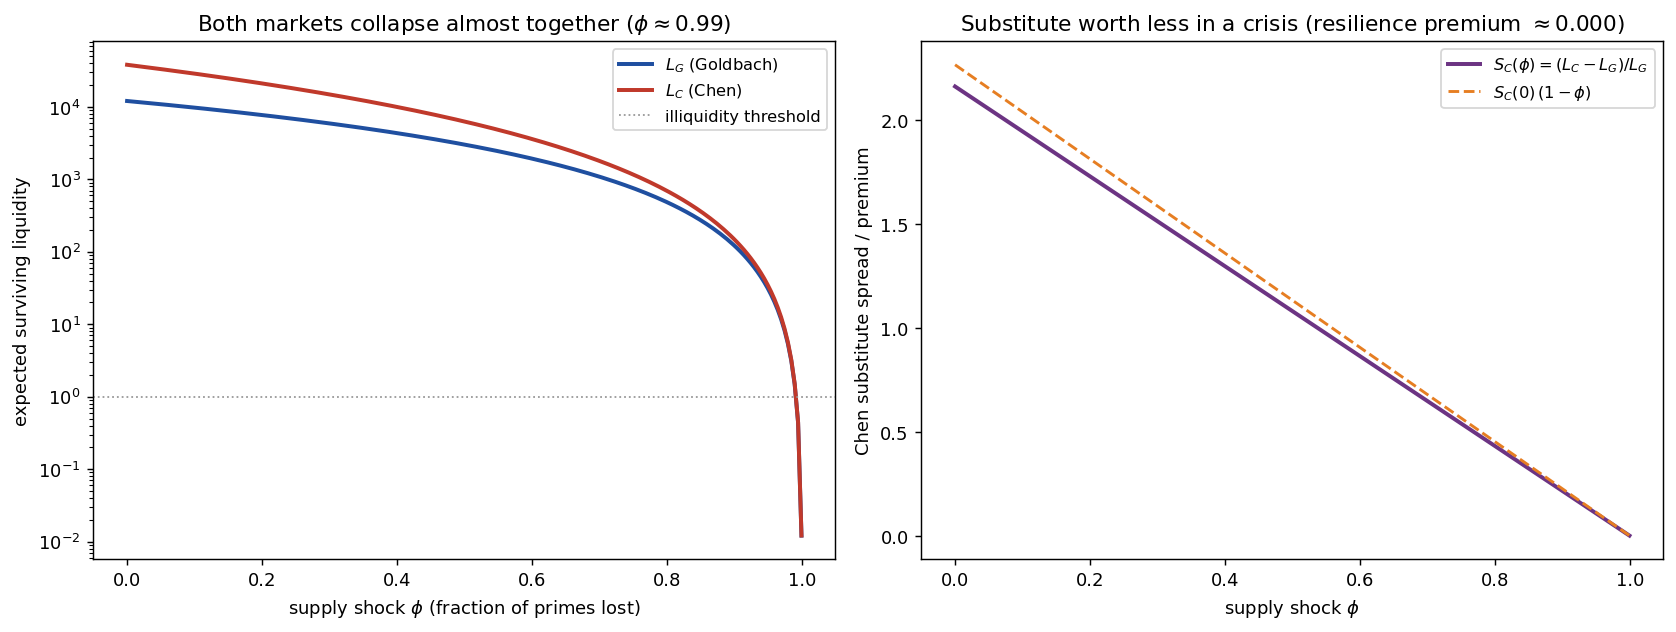
\includegraphics[width=\linewidth]{19_mercado.png}
\caption{Goldbach as a market under a prime supply shock $\phi$. Left: expected surviving
liquidity of the Goldbach and Chen markets, both crossing the illiquidity threshold near
$\phi=0.99$. Right: the Chen substitute spread $S_C(\phi)=S_C(0)(1-\phi)$ vanishes
linearly---no resilience premium.}
\label{fig:market}
\end{figure}

\section{Persistent topology of additive decompositions (a negative note)}
\label{sec:tda2}

It is tempting to filter additive decompositions of $N$ by arithmetic complexity rather
than geometric distance: form the complex
$K_N^{(k)}=\{\{a,b\}:a+b=N,\ \OmegaF(a)+\OmegaF(b)\le k\}$ and let $k$ grow. But for the
\emph{binary} problem this is topologically empty: each integer $a$ lies in the single
pair $\{a,N-a\}$, so $K_N^{(k)}$ is a disjoint matching for every $k$. Its $0$-dimensional
persistence is therefore exactly the energy spectrum of \S\ref{sec:energy-emp}---each pair
is a component born at its energy $\OmegaF(a)+\OmegaF(b)$ and never dying---and all higher
homology vanishes. There is no topological structure to discover beyond the spectrum.

Genuine higher dimension appears only at the \emph{ternary} level. For odd $N$, form the
graph on primes $p<N$ with an edge $\{p,q\}$ whenever $N-p-q$ is prime, so that each edge
\emph{is} a ternary representation $(p,q,N-p-q)$. At $N=99{,}999$ this graph has $9{,}591$
vertices and $3.9\cdot10^{6}$ edges (density $0.084$, minimum degree $2$, so it is
connected---a graph form of Helfgott's ternary theorem). Yet it is strongly
\emph{anti}-clustered: it contains far fewer triangles than a random graph of equal
density, so ternary representations do not aggregate into higher-order simplices. The
honest conclusion is that the additive-complexity filtration adds nothing to the spectral
and graph-theoretic pictures already developed; we record it as a negative result.

\section{Goldbach as control: the value of arithmetic information}
\label{sec:control-emp}

Finally, view the even integers as a sequence of markets to be cleared by a controller: at
each $N$ the controller picks a prime $p$ (the action) and clears if $q=N-p$ is prime.
Goldbach is the statement that a successful policy exists; the computational question is
which \emph{simple} policy clears fastest. A naive policy ignores the arithmetic of $N$; a
\emph{residue-aware} policy with information budget $B$ uses the residues $N\bmod\ell$ for
primes $\ell\le B$ to prefer $p$ with $N-p$ coprime to those $\ell$---i.e.\ it avoids
spending tries on partners forced to share a small factor. Over a window near $10^{6}$
(Fig.~\ref{fig:control}), the single-shot clearing probability rises from $18\%$ (naive) to
$39\%$ at $B=13$, and the expected number of tries in a sequential search falls from $5.5$
to $2.5$---a $55\%$ reduction. The marginal value of each prime of information is largest at
$\ell=3$ (the factor $\tfrac{\ell-1}{\ell-2}=2$) and decreases thereafter, exactly tracking
the singular series. Unlike the other reframings in this section, this one yields a
concrete \emph{algorithm} rather than a restatement: the residue-aware ordering is a drop-in
search heuristic---enumerate candidate $p$ in increasing order of the number of small primes
$\ell\le B$ that $N-p$ is forced to share with $N$---whose benchmark above (expected tries
$5.5\to2.5$ at $B=13$, a $55\%$ reduction) is a measured speed-up of the per-$N$ Goldbach
search---the cost of finding one representation for a given $N$, distinct from the global
verification $R_1>0$ for all $N\le X$, which the FFT already settles---not an analogy. The same local arithmetic the singular series encodes is thus directly
actionable.

\begin{figure}[h]
\centering
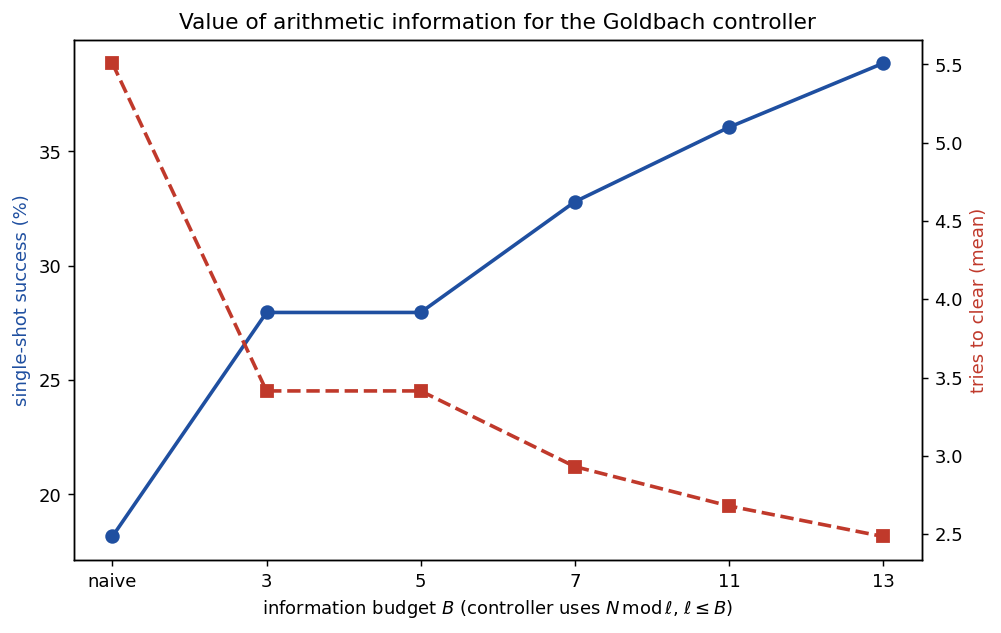
\includegraphics[width=0.66\linewidth]{20_control.png}
\caption{Value of arithmetic information for the Goldbach controller. As the information
budget $B$ grows, the single-shot clearing probability (blue) rises and the sequential
clearing cost (red) falls; the gain per prime tracks the singular-series factor
$(\ell-1)/(\ell-2)$.}
\label{fig:control}
\end{figure}

\section{The information content of the comet}
\label{sec:info-emp}

The spectral saturation invites an information-theoretic reading: how compressible is the
comet, and what is irreducible? Decomposing the variance of $\log R_1(N)$ into a smooth
trend, the local arithmetic (the conditional mean given $N\bmod30030$, which captures
$\sing$ non-linearly), and a residual, we find (Fig.~\ref{fig:info})
\[
  \underbrace{81.1\%}_{\text{trend }N/\log^2N}\ +\ \underbrace{18.8\%}_{\text{singular series }\sing(N)}\ +\ \underbrace{0.11\%}_{\text{irreducible}} .
\]
The comet is thus $99.9\%$ compressible \emph{by this particular code}---the conditional
mean given $N\bmod30030=2\cdot3\cdot5\cdot7\cdot11\cdot13$. We stress that this figure is
relative to the chosen conditioning set, not a theorem: the ``irreducible'' $0.11\%$ is
what survives after removing structure up to the prime $13$, and a richer conditioning
(more primes, or non-residue features) would shrink it further. With that caveat, the
residual is informative: its power spectrum is \emph{flat}---white noise, in contrast to
the sharply peaked spectrum of $R_1$ itself (the empirical circle method of the main text)---with lag-$1$
autocorrelation $-0.04$ and standard deviation $2.7\%$, a few times the Poisson floor
$\langle R_1\rangle^{-1/2}=0.9\%$. So \emph{up to modulus $30030$} the Goldbach comet is
almost entirely a singular-series codeword and the residue carries no further \emph{small-modulus}
arithmetic signal; we do not claim the absence of all further structure, only that none is
visible below this conditioning.

\begin{figure}[h]
\centering
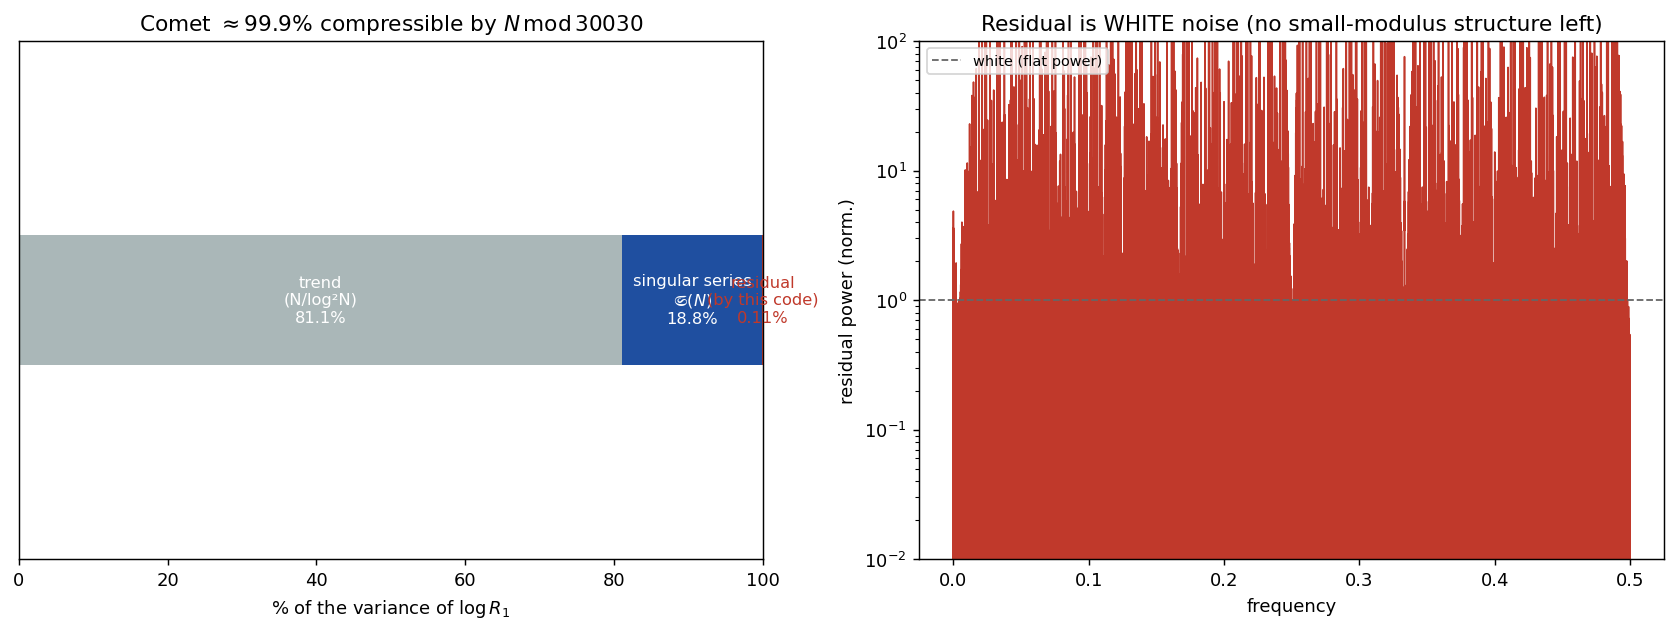
\includegraphics[width=\linewidth]{22_informacion.png}
\caption{Information budget of the comet \emph{relative to conditioning on $N\bmod30030$}.
Left: the variance of $\log R_1$ splits into a smooth trend ($81\%$), the singular series
($18.8\%$), and a residual ($0.11\%$) that is irreducible \emph{by this code} (richer
conditioning would shrink it). Right: the residual's power spectrum is flat---white noise,
with none of the small-modulus arithmetic peaks seen in the main text's comet spectrum.}
\label{fig:info}
\end{figure}

\section{Discrete geometry of the Chen surface}
\label{sec:geom-emp}

Each Chen representation $N=p+rs$ ($q=N-p$ semiprime, $r=\mathrm{spf}(q)\le s$) is a lattice
point on the surface $p+rs=N$. In normalised logarithmic coordinates
$u=\log r/\log N,\ v=\log s/\log N$ the points fill the triangle $\{u\le v,\ u+v\le1\}$,
with the edge $u=0$ (i.e.\ $r$ bounded) the Goldbach boundary and the diagonal $u=v$ the
balanced semiprimes. Accumulating $6.6\cdot10^{7}$ solutions over a window near $10^{6}$
(Fig.~\ref{fig:geom}, left) shows a cloud organised into discrete vertical \emph{rays}---one
for each small prime $r=3,5,7,\dots$, since $r$ is prime---whose brightness decreases with
$r$: the mass piles up against the Goldbach edge.

Quantitatively, the Li--Liu exponent of a solution, $a=1+\log r/\log s$, has the spectrum of
Fig.~\ref{fig:geom} (right): it peaks near $a\approx1.1$ and decays toward the balanced
value $2$, with mean $1.38$ and \emph{median $1.30$}. Half of all Chen solutions already
satisfy $a<1.3$, and essentially all sit far below the uniform threshold $a=1.9$ of
Li--Liu. So the Chen solutions of a typical $N$ concentrate near the Goldbach boundary: the
semiprime second summand is, far more often than not, an unbalanced product with a small
factor---the geometric form of the residual-exponent and factor-balance findings of
the main text.

\begin{figure}[h]
\centering
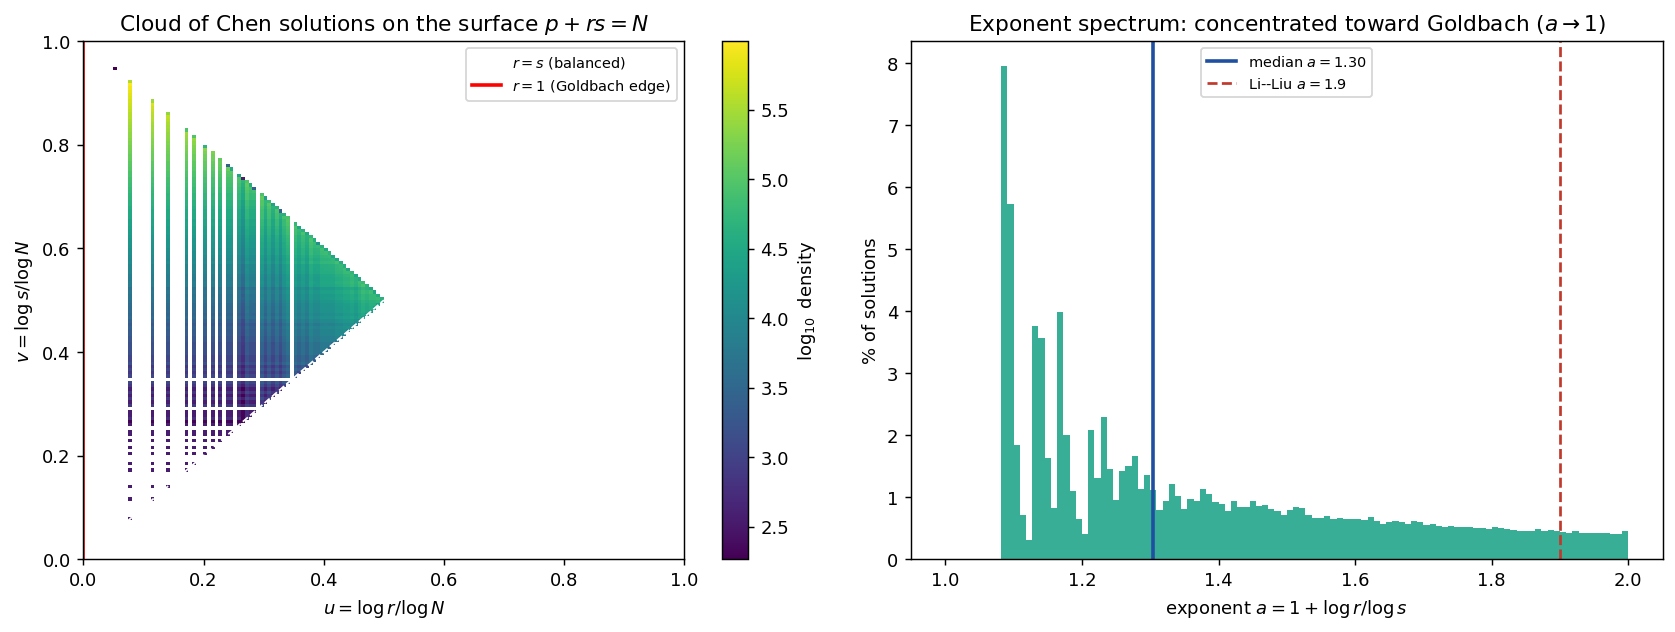
\includegraphics[width=\linewidth]{23_geometria.png}
\caption{Discrete geometry of $p+rs=N$. Left: density of Chen solutions in
$(u,v)=(\log r/\log N,\log s/\log N)$, with discrete rays at each prime $r$ and mass against
the Goldbach edge $u=0$. Right: the exponent spectrum $a=1+\log r/\log s$, median $1.30$,
far below the Li--Liu threshold $1.9$.}
\label{fig:geom}
\end{figure}


\end{document}
